\chapter{Theory} 
\label{ch:theory}

\minitoc

%What's the standard model all about? 

%\section{In the beginning...}
%\section{Some other stuff}



%\section{The Standard model of Particle of Physics}
\section{The weak force in \bquark-hadron decays}

Ground state \bquark-hadrons can only decay via the weak interaction as the \bquark must change flavour to one of the first or second generation quarks.
These decays were first observed ... with lifetime ...
Although the weak interaction dictates the core of the process, the contributions from the strong force are unavoidable. In the SM quarks abide by \emph{confinement}, preventing bare quarks from propagating unhindered. Instead quarks are only ever observed in bound states, or hadrons, with other quarks or anti-quarks. Therefore the observation of the weakly decaying \bquark-quark is necessarily accompanied by the strong interaction governing the hadronisation of the initial and final state quarks.


\subsection{The weak force}

The weak interaction differs remarkably from the electromagnetic and strong interactions. It is the only of the three to be mediated by massive gauge bosons and violates parity; the action of mirroring space. 
Additionally, there are two types of gauge boson: the charged \Wpm bosons that result in \emph{charged-current} interactions; and the neutral \Z boson, responsible for \emph{neutral-current} interactions. 

Confusingly, the weak interaction is actually stronger than the electromagnetic force, however the large mass of the mediators suppresses the interaction at low energy.
The \emph{charged-current} weak interaction was originally described by Fermi using a four point coupling $G_{\text{F}}$. This works well for low energy interactions in which the momentum transfer is much less than the \Wpm boson mass, $|q^{2}|<<m_\Wpm^2$. In the higher mass range this breaks down leading to unitarity violation in processes such as \decay{\ep\en}{\Wp\Wm}. This is resolved by the addition of the neutral \Z boson and the \emph{neutral-current} interactions that restore unitarity. 



{\color{Red}
\begin{itemize}
\item Hyper charge
\item couplings
\end{itemize}}



\subsubsection{Parity violation}
Parity is conserved in QCD and QED so it was naturally assumed to follow suit in the weak interaction. In 1957 is was shown by C.S. Wu and collaborators that parity was indeed violated in the beta decay of cobalt-60~\cite{PhysRev.105.1413}. The rate of electrons emitted during the decay were measured as a function of the polar angle. In the parity conservation scenario the same rates would have been expected at angles of $\theta$ and $180^\circ-\theta$ to an applied magnetic field; however electrons are preferably emitted against the field.          

The weak interaction can be described as a V-A interaction (vector-axialvector), corresponding to a maximally parity violating interaction. In the ultra-relativistic limit this would mean that the weak force only couples to left-handed particles and right-handed antiparticles. {\color{Red} define helicity?} This is relaxed when accounting for the non-zero masses of fermions, but leads to helicity suppression for certain processes, for example \decay{\pim}{\en\neueb} with respect to \decay{\pim}{\mun\neumb}. The relative branching fractions for these two processes acts as strong experimental evidence for the V-A interaction.

\subsubsection{Electroweak unification}

Although the weak and electromagnetic forces can be described by QED and the Fermi interaction at low energies, this becomes insufficient at high energies. Here, the weak and electromagnetic forces can be unified through the single Electroweak gauge theory with a $\text{SU}(2)_{L}\times\text{U}(1)_{Y}$ symmetry.

The \Z boson introduced to prevent unitarity violation is experimentally observed to couple to both left-handed and right-handed particles, in contrast to the \Wpm boson. This seemingly contradictory situation was resolved by Glashow, Salam and Weinberg~\cite{Glashow:1959wxa,Salam:1968rm,Weinberg:1967tq} who developed a unification of the electromagnetic and weak interactions. 
This begins by replacing the physical electromagnetic $\text{U}(1)_{\text{Q}}$ interaction with a similar $\text{U}(1)_{\text{Y}}$ interaction that couples to weak hyper-charge, $Y$. This gauge symmetry requires a new gauge boson $B$. The weak $\text{SU}(2)_{L}$ interaction generates three gauge bosons. The third of these, $W^{3}$, can mix with the new $B$ gauge boson to generate the two physical bosons $\gamma$ and \Z
\begin{equation}
\left( \begin{array}{c} \gamma \\ \Z \end{array} \right) = \begin{pmatrix} \cos{\theta_{W}} & \sin{\theta_{W}} \\ -\sin{\theta_{W}} & \cos{\theta_{W}} \end{pmatrix} \left( \begin{array}{c} B \\ W^{3} \end{array} \right),
\end{equation}
where $\theta_{W}$ is the weak mixing angle. 

{\color{Red}
\begin{itemize}
\item Photon and Z mix
\end{itemize}}


\subsection{Weak interactions of quarks}

The weak force couples to quarks 


{\color{Red}
\begin{itemize}
\item semileptonic decays 
\item cabibbo formulated angle
\item  
\end{itemize}}


\subsection{The CKM matrix}

\begin{equation}
\left( \begin{array}{c} d' \\ s'  \\ b' \end{array} \right) = \begin{pmatrix} \Vud & \Vus & \Vub \\ \Vcd & \Vcs & \Vcb  \\ \Vtd & \Vts & \Vtb \end{pmatrix} \left( \begin{array}{c} d \\ s  \\ b \end{array} \right)
\end{equation}


\begin{equation}
\left( \begin{array}{c} d' \\ s'  \\ b' \end{array} \right) = \begin{pmatrix} 1 - \lambda^2/2 & \lambda & A\lambda^3(\rho-i\eta) \\ -\lambda & 1-\lambda^2/2 & A\lambda^2  \\ A\lambda^3(1-\rho-i\eta) & -A\lambda^2 & 1 \end{pmatrix} \left( \begin{array}{c} d \\ s  \\ b \end{array} \right)
\end{equation}


{\color{Red}
\begin{itemize}
\item introduce idea of CP violation
\item Observation of CP violation? 
\end{itemize}}

\subsection{\bquark-hadron physics}
The b stands for beauty
{\color{Red}
\begin{itemize}
\item CP violation in the B sector
\item \B meson mixing
\item lifetime maybe? 
\end{itemize}}

\subsection{QCD and hadronisation}
{\color{Red}
\begin{itemize}
\item Explain why predictions are hard
\item lattice QCD
\item light cone sum rules? 
\end{itemize}}

\section{Annihilation topology decays}

{\color{Red}
\begin{itemize}
\item Talk about \D and other annihilation topologies 
\item Find origin of hadronic uncertainties 
\end{itemize}}


\subsection{Pure annihilation topology decays}
{\color{Red}
\begin{itemize}
\item Pure annihilation - charmless Bc
\end{itemize}}
\subsection{Other annihilation decays}

{\color{Red}
\begin{itemize}
\item non pure - donals Bc 
\end{itemize}}

\section{Rescattering}

{\color{Red}
\begin{itemize}
\item What is rescattering?
\item Examples of it?
\item Why it's expected to be small
\end{itemize}}

\section{Theoretical predictions for the \decay{\Bp}{\Dsp\phiz} decay}

%%%%%%%%%%%%%%%%%%%%%%%%%%%%%%%%%%%%%%%%%%%%%%%%%%%%%%%%%%
\begin{figure}[!h]
    \centering
    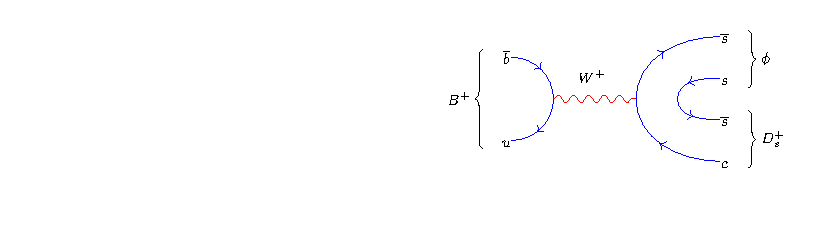
\includegraphics[width=0.6\textwidth]{figs/Theory/B2DsPhi.pdf}
    \caption{\decay{\Bp}{\Dsp\phiz} }
    \label{fig:Theory_DsPhiDiagram}   
\end{figure}
%%%%%%%%%%%%%%%%%%%%%%%%%%%%%%%%%%%%%%%%%%%%%%%%%%%%%%%%%%



{\color{Blue}
In the SM, the decay $\decay{\Bp}{\Dsp\phi}$ proceeds dominantly via the annihilation diagram shown in Fig.~\ref{fig:Theory_DsPhiDiagram}. 
This suppressed topology requires the wave functions of the incoming quarks to overlap sufficiently to annihilate into a virtual \Wp boson. 
The decay is further suppressed by the small magnitude of the CKM matrix element \Vub associated with the annihilation vertex. 


}

\subsection{Standard model predictions}
{\color{Blue}
Several SM predictions have been made for the branching fraction of the $\decay{\Bp}{\Dsp\phi}$ decay~\cite{Zou:2009zza, Mohanta:2002wf, Mohanta:2007uu, Lu:2001yz}, using input from lattice calculations~\cite{fB:2013HPQCD,fB:2016ETM, fB:2016Fermi}. These predictions are in the range $(1-7)\times10^{-7}$, where the limit on the precision is dominated by hadronic uncertainties. 

In addition, unlike many rare hadronic decays including $\decay{\Bp}{\Dsp\Kp\Km}$, possible contributions from rescattering effects are expected to be small, for example contributions from intermediate states such as $\decay{\Bp}{\Dsp\omega}$~\cite{Gronau:2012gs}.

}

{\color{Red}
\begin{itemize}
\item Find origin of hadronic uncertainties 
\end{itemize}}

\subsection{BSM models and predictions}
{\color{Blue}
However, additional diagrams contributing to this decay can arise in some extensions of the SM, such as supersymmetric models with R-parity 
violation. They could enhance the branching fraction and/or produce large \CP asymmetries~\cite{Mohanta:2002wf, Mohanta:2007uu}, which makes the $\decay{\Bp}{\Dsp\phi}$ decay a promising place to search for new physics beyond the SM.\footnote{Charge conjugation is implied throughout this paper. Furthermore, $\phi$ denotes the $\phi(1020)$ resonance.}
}

{\color{Red}
\begin{itemize}
\item Higgs doublet
\item SUSY 
\item include feynman diagrams
\item small intro into models
\end{itemize}}

\subsection{Previous measurements}

{\color{Blue}
The \lhcb experiment reported evidence for the decay $\decay{\Bp}{\Dsp\phi}$ using $pp$ collision data corresponding to an integrated luminosity of 1\invfb taken during 2011, at a centre-of-mass energy of 7\tev~\cite{Aaij:2012zh}. A total of $6.7^{+4.5}_{-2.6}$ candidates was observed. The branching fraction was determined to be 

\begin{equation}
\mathcal{B}(\decay{\Bp}{\Dsp\phi}) = (1.87^{+1.25}_{-0.73} \pm 0.19 \pm 0.32) \times 10^{-6},
\end{equation}
where the first uncertainty is statistical, the second is systematic and the third is due to the uncertainty on the branching fraction of the decay $\decay{\Bp}{\Dsp\Dzb}$, which was used as normalisation. 
Given the large uncertainties on both the theoretical and experimental values, the previously measured value is consistent with the range of SM values given above.
}

{\color{Red}
\begin{itemize}
\item Include plot and measurement
\item say something about similarites 
\end{itemize}}


\section{Theoretical predictions for the \decay{\Bp}{\Dsp\Kp\Km} decay}


%%%%%%%%%%%%%%%%%%%%%%%%%%%%%%%%%%%%%%%%%%%%%%%%%%%%%%%%%%
\begin{figure}[!h]
    \centering
    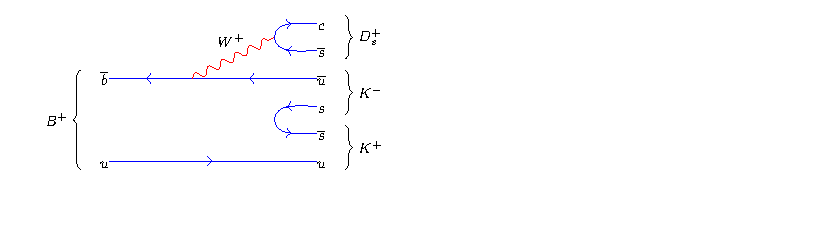
\includegraphics[width=0.6\textwidth]{figs/Theory/B2DsKK.pdf}
    \caption{\decay{\Bp}{\Dsp\Kp\Km} }
    \label{fig:Theory_DsKKDiagram}   
\end{figure}
%%%%%%%%%%%%%%%%%%%%%%%%%%%%%%%%%%%%%%%%%%%%%%%%%%%%%%%%%%



{\color{Blue}
The decay $\decay{\Bp}{\Dsp\Kp\Km}$ is mediated by a $\decay{\bquarkbar}{\uquarkbar}$ transition shown in Fig.~\ref{fig:Theory_DsKKDiagram} and is therefore suppressed in the Standard Model (SM) due to the small size of the Cabibbo-Kobayashi-Maskawa (CKM) matrix element \Vub. 
}


{\color{Red}
\begin{itemize}
\item explain what a dalitz plot is
\end{itemize}
}

\subsection{Standard model predictions}
{\color{Blue}
The branching fraction for this decay is currently not measured, however a similar decay, \decay{\Bp}{\Dsp \piz}, has been observed with a branching fraction of $\mathcal{B}(\decay{\Bp}{\Dsp \piz}) = (1.5 \pm 0.5) \times 10^{-5}$~\cite{Aubert:2006xy}.
}


{\color{Red}
\begin{itemize}
\item talk about \decay{\Bp}{\Dsp\piz}
\item Could talk about \decay{\Bp}{\Dp\Kp\pim} and estimate   
\end{itemize}}

\subsection{Previous measurements}



